\documentclass[acmsmall,screen,review,anonymous]{acmart}
\usepackage{amsmath,amssymb,amsfonts}
\usepackage{algorithmic}
\usepackage{graphicx}
\usepackage{textcomp}
\usepackage{xcolor}
\usepackage{booktabs}
\usepackage[skins]{tcolorbox}
\usepackage{multirow}
\usepackage{listings}
\usepackage{colortbl}
\usepackage{array}
\usepackage{pifont}
\usepackage{pgfplots}
\usepackage{threeparttable}
\usepackage{placeins}
% \usepackage[numbers,sort&compress]{natbib} # this will make the font size of references larger (may be some bugs)
\usepackage{arydshln}
\usepackage{xspace}
\usepackage{enumitem}
\usepackage{makecell}
\newcommand{\ourmethod}{ABC\xspace}
\newcommand{\cmark}{\ding{51}}
\newcommand{\xmark}{\ding{55}}
\newcommand{\todoc}[2]{{\textcolor{#1}{\textbf{[#2]}}}}
\newcommand{\todoblue}[1]{\todoc{blue}{\textbf{#1}}}
\newcommand{\todored}[1]{\todoc{red}{\textbf{#1}}}
\newcommand{\yin}[1]{\todoblue{yin: #1}}
\newcommand{\gu}[1]{\todored{gu: #1}}
\newcommand{\shen}[1]{\todored{shen: #1}}
\setlength{\textfloatsep}{10pt plus 2pt minus 2pt}
\setlength{\floatsep}{8pt plus 2pt minus 2pt}
\setlength{\intextsep}{9pt plus 2pt minus 2pt}
\setlength{\dbltextfloatsep}{10pt plus 2pt minus 2pt}
\setlength{\dblfloatsep}{8pt plus 2pt minus 2pt}
\begin{document}

\title{Reasoning Patterns for Efficient AI Coding: An Empirical Study
}
%Reasoning Patterns Matter: An Empirical Study of LLM Coding for Inference Efficiency
%Reasoning Patterns in AI Coding: An Empirical Study and Pattern-Aware Inference Efficiency

\author{Anonymous Author(s)}

\begin{abstract}
Large Reasoning Models (LRMs) increasingly produce long reasoning traces that are used not only to explain model decisions but also to guide prompting, self-refinement, and inference-time control. However, their underlying reasoning patterns in AI coding tasks remain poorly understood, limiting systematic analysis and optimization. 
We conduct an empirical study of reasoning patterns in AI coding by transforming reasoning traces into action sequences and mining reusable patterns at two levels: macro patterns that capture task-level reasoning strategies, and micro patterns that distinguish valid from invalid reasoning behaviors at a finer granularity. Our findings show that each coding task exhibits a distinct macro pattern reflecting its underlying problem-solving strategy; for example, code generation follows a design-to-implementation flow, whereas debugging follows an evidence–fix–recheck loop. At the micro level, valid traces exhibit verification-driven convergence, while invalid traces are characterized by anti-patterns such as repeated design revision, reflection, and knowledge recall without closure.
We further demonstrate the utility of these patterns through three applications. Macro-pattern features enable accurate task identification from reasoning traces. Micro-pattern-guided prompting improves single-attempt correctness with comparable token cost, while anti-pattern-aware early stopping reduces reasoning tokens by 30–69\% while maintaining competitive accuracy. These gains generalize across unseen models, indicating that the identified patterns are robust and model-agnostic.
\end{abstract}

\keywords{reasoning patterns, AI coding, reasoning trace analysis,
reasoning pattern mining, inference-time optimization}

\maketitle

\section{Introduction}

Large reasoning models (LRMs) are rapidly reshaping AI coding~\cite{codethinksurvey,sweagent2024}. Unlike conventional code language models that directly generate outputs, LRMs explicitly produce multi-step reasoning before arriving at a solution. This capability is particularly valuable for coding tasks, which often require structured intermediate reasoning, such as algorithm design in code generation and state tracking in program execution reasoning. Consequently, reasoning has become a first-class component of coding performance rather than a by-product of final answers.

The availability of explicit reasoning traces has enabled extensive research on their role in code-related reasoning and generation~\cite{wei2022cot,deepseekr1}. Prior work shows that reasoning traces can significantly influence coding outcomes, but they also introduce inefficiencies, including incorrect intermediate assumptions, redundant exploration, repetitive reflections, and excessive deliberation that increases inference cost without improving correctness~\cite{revisitcotcodegen,cotcodequality,thinkingpatterns,overthinking2025}. 
Reasoning traces have therefore been increasingly exploited beyond explanation, supporting self-correction~\cite{reflexion,selfrefine}, evaluation~\cite{codevisionary2025,judgeuncertainty2025}, and inference-time control~\cite{seer2025,turncontrol2025}.

Despite these advances, existing work primarily focuses on final task performance~\cite{codex,livecodebench,swebench2024}, prompting strategies~\cite{wei2022cot,selfconsistency,codecot}, or isolated reasoning behaviors in specific coding tasks (e.g., code generation)~\cite{revisitcotcodegen,cotcodequality,thinkingpatterns,reasoningsteps2026}, rather than treating reasoning traces as structured, recurring regularities across instances and tasks.
As a result, the higher-level organizational structure of reasoning in AI coding remains underexplored. 
In particular, it is still unclear whether LRMs exhibit stable reasoning patterns across tasks, what distinguishes effective from ineffective reasoning trajectories, and how such patterns relate to reasoning efficiency and correctness.

To address this gap, we conduct an empirical study of reasoning patterns in AI coding. We collect reasoning traces generated by LRMs on four representative coding tasks (i.e., code generation, code execution reasoning, program debugging, and code translation) and transform them into structured reasoning action sequences using a unified action taxonomy. This abstraction enables us to move beyond unstructured textual traces and analyze reasoning as structured behavioral processes. Based on this representation, we study the structure, effectiveness, and practical utility of reasoning patterns across tasks and models.

Specifically, we investigate the following research questions:

\begin{itemize}[itemsep=1.5mm]

\item \textbf{RQ1 (Macro Patterns): What task-level reasoning patterns emerge across different coding tasks?}

Different coding tasks impose distinct reasoning demands, yet it remains unclear whether LRMs develop consistent task-level reasoning structures. To characterize these structures, we segment reasoning traces into action sequences using a predefined taxonomy and mine recurring action-fragment signatures across four coding tasks, yielding a high-level view of how reasoning strategies differ across tasks.

\item \textbf{RQ2 (Micro Patterns): What fine-grained reasoning patterns distinguish valid and invalid reasoning trajectories?}

Beyond task-level structures, reasoning quality is largely shaped by fine-grained dynamics within trajectories. We therefore mine positive and anti-patterns from valid and invalid reasoning traces to capture local mechanisms that facilitate or hinder problem solving. For tasks with objective correctness signals, we assess trace validity using an ensemble LLM-as-a-judge protocol and extract micro patterns via trace measurement and frequent fragment mining.

\item \textbf{RQ3 (Applications): How can discovered reasoning patterns be leveraged to improve AI coding performance?}

If reasoning patterns reflect stable and generalizable structure, they should be useful beyond analysis, enabling improvements in inference-time behavior. To this end, we study three applications: task identification from macro-pattern features, prompting augmentation with micro-pattern guidance, and inference-time efficiency improvement via anti-pattern-triggered early stopping.

\end{itemize}

Our study yields three main findings. First, each coding task exhibits a distinct macro-level reasoning structure: code generation follows a design-to-implementation flow, code execution reasoning relies on state tracing, debugging proceeds via an evidence–fix–verification loop, and code translation centers on semantic mapping. Second, valid and invalid trajectories diverge in their micro-level dynamics: valid traces show verification-driven convergence, whereas invalid traces exhibit repeated redesign, reflection, and knowledge recall without resolution. Third, these patterns are actionable: they enable accurate task identification, improve single-shot correctness via pattern-guided prompting, and reduce reasoning tokens by 30–69\% via anti-pattern-aware early stopping while preserving competitive accuracy.

In summary, this paper makes the following contributions:

\begin{itemize}[itemsep=1.5mm]

\item We present the first empirical study of reasoning patterns in cross-task AI coding, introducing a reasoning-action representation that transforms free-form reasoning traces into structured action sequences for analysis.

\item We identify both macro- and micro-level reasoning patterns across four representative coding tasks, revealing task-specific reasoning strategies as well as recurring fine-grained patterns and anti-patterns associated with valid and invalid reasoning trajectories.

\item We show that reasoning patterns constitute an actionable abstraction for LRM-based AI coding, and demonstrate their utility in task identification, pattern-guided prompting, and anti-pattern-aware early stopping, improving both interpretability and inference efficiency.

\end{itemize}

\section{Methodology}  

%\subsection{Study Overview}

\begin{figure*}[h]
\centering
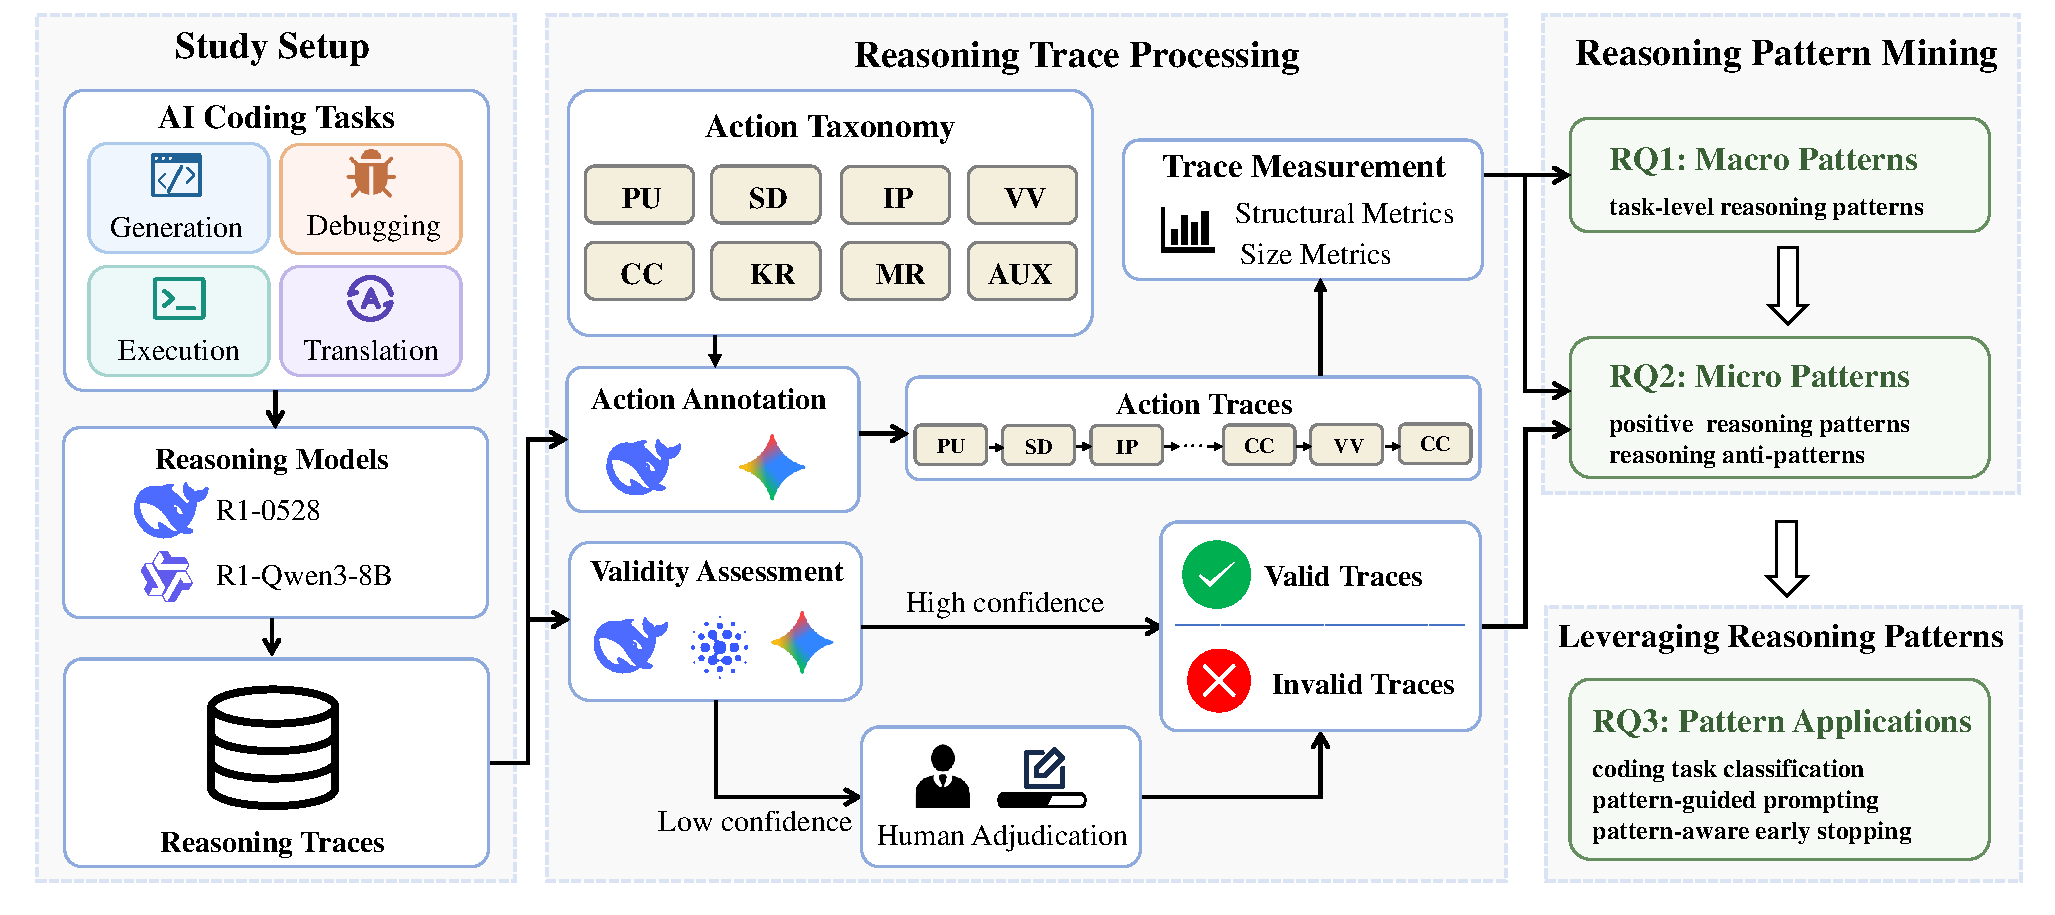
\includegraphics[width=0.95\textwidth]{figures/framework.pdf}
\caption{Overview of the reasoning-pattern analysis framework.}
\label{fig:overview}
\end{figure*}


Figure~\ref{fig:overview} illustrates the process of our empirical study.
First, we collect reasoning traces from two LRMs on four representative AI coding tasks (\S\ref{sec:study-setup}) and assess the validity of each trace. 
Second, guided by the reasoning-action taxonomy, we annotate each reasoning trace into an action trace and quantify reasoning behaviors using action- and trace-level metrics (\S\ref{sec:trace-processing}). 
Third, we mine recurring reasoning patterns from the resulting action traces (\S\ref{sec:pattern-mining}), covering task-level macro patterns (RQ1) and validity-related micro patterns and anti-patterns (RQ2). 
Finally, RQ3 explores how the discovered reasoning patterns can be leveraged for AI coding (\S\ref{sec:pattern-applications}), including coding task classification, pattern-guided prompting, and pattern-aware early stopping.

\subsection{Study Setup}
\label{sec:study-setup}

%\subsubsection{Task and Dataset Selection}
To investigate reasoning patterns in AI coding, we study four representative coding tasks that cover program synthesis, comprehension, maintenance, and transformation:

\begin{itemize}[itemsep=1.5mm]

\item \textit{Code generation}, which requires a model to synthesize executable programs from natural-language specifications.
We use LiveCodeBench v4--v6~\cite{livecodebench}, comprising 442 instances.

\item \textit{Code execution reasoning}, which requires a model to infer the output of a program through static reasoning rather than actual execution.
We use the input--output prediction subset of CodeSense~\cite{codesense}, comprising 382 instances.

\item \textit{Program debugging}, which requires a model to localize and repair defects in buggy programs.
We use DebugBench~\cite{debugbench}, comprising 500 instances.

\item \textit{Code translation}, which requires a model to transform programs across programming languages while preserving their semantics.
We use ClassEval-T~\cite{classeval-t}, comprising 376 instances.

\end{itemize}

These tasks all provide objective correctness oracles, which allow us to analyze both reasoning traces and task outcomes under a unified experimental setting.

%\subsubsection{Models}
We evaluate two publicly available LRMs: DeepSeek-R1-0528 (denoted as R1-0528) and DeepSeek-R1-0528-Qwen3-8B (denoted as R1-Qwen3-8B)~\cite{deepseekr1}. R1-Qwen3-8B is obtained by distilling R1-0528 into a Qwen3-8B backbone. For every task instance, both models are evaluated using identical prompts and decoding configurations. We collect each model's complete reasoning trace together with its final response, forming the dataset used in the subsequent analyses.

\subsection{Reasoning Trace Processing}
\label{sec:trace-processing}

This section describes how we process the collected reasoning traces into reasoning action traces and the derived metrics used for subsequent reasoning pattern mining and analysis.

\subsubsection{\textbf{Reasoning Trace Collection}}
For each task instance, we instantiate the benchmark-provided prompt template with instance-specific inputs (e.g., problem description, starter code, buggy program, or source-language snippet), and submit it independently to each model in thinking mode under a unified sampling configuration (temperature \(=0.6\), top-\(p=0.95\)).

We extract the content enclosed by the \texttt{<think>} tags as the reasoning trace. To ensure completeness, we regenerate any response with an empty reasoning trace or lacking the information required for annotation or task evaluation, until a complete trace and task output are obtained.

After filtering incomplete, unparsable, or unlabeled responses, the resulting dataset contains 3{,}376 reasoning traces across the four tasks and two models: 442/440 traces for code generation, 377/378 for code execution reasoning, 499/496 for debugging, and 372/372 for code translation on R1-0528/R1-Qwen3-8B, respectively. %In total, R1-0528 contributes 1{,}690 traces and R1-Qwen3-8B contributes 1{,}686 traces.

\subsubsection{\textbf{Reasoning Trace Validity Assessment}}
To compare valid and invalid reasoning behaviors in RQ2, we assess the validity of each reasoning trace using an ensemble LLM-as-a-judge protocol~\cite{llmjudge,customizedevaluator}. Trace-level validity is distinct from task-level functional correctness: a response may produce a correct final answer while its reasoning trace still contains logical inconsistencies or unnecessary reasoning detours. A reasoning trace is considered \emph{valid} if its reasoning is internally consistent and progresses coherently toward the final solution.

We employ three judge models, DeepSeek-V3.2~\cite{deepseekv32}, Gemini-3-Flash~\cite{gemini3flash}, and GLM-5.1~\cite{glm51}, each independently classifying a trace as \emph{valid} or \emph{invalid}. To reduce judgment variance, each judge is queried three times, returning a binary label \(y_{m,r}\in\{\mathrm{valid},\mathrm{invalid}\}\) with a confidence score \(c_{m,r}\in[0,1]\).

We aggregate the nine judgments using confidence-weighted voting:

\begin{equation}
S(\ell)=
\frac{\sum_{m\in\mathcal{M}}\sum_{r=1}^{3} c_{m,r}\cdot \mathbf{1}[y_{m,r}=\ell]}
{\sum_{m\in\mathcal{M}}\sum_{r=1}^{3} c_{m,r}},
\end{equation}
where \(S(\ell)\) denotes the normalized confidence-weighted support for label \(\ell\). The final label is assigned as
\(\hat{y}=\arg\max_{\ell}S(\ell)\), with confidence \(\max_{\ell}S(\ell)\). We automatically accept the aggregated label when its confidence exceeds 0.8; otherwise, the reasoning trace is adjudicated by two human annotators. The resulting labels define the valid and invalid reasoning-trace groups. In total, the dataset contains 2{,}452 valid traces and 924 invalid traces: R1-0528 contributes 1{,}439 valid and 251 invalid traces, while R1-Qwen3-8B contributes 1{,}013 valid and 673 invalid traces. 

\subsubsection{\textbf{Reasoning Action Taxonomy and Annotation}}
Reasoning traces are free-form natural-language text, making systematic comparison across tasks and models difficult. To enable structured analysis, we represent each reasoning trace as a sequence of fine-grained \textit{reasoning actions}, where a reasoning action is defined as a contiguous text span expressing a distinct reasoning behavior.

Drawing on prior studies of LLM reasoning~\cite{codethinksurvey,thinkingpatterns,reflexion,selfrefine}, we define a taxonomy of eight reasoning actions that captures the major stages of code reasoning, ranging from task understanding and solution construction to verification and reflection. To strengthen its validity, the taxonomy is further inspected by two researchers with over five years of experience in code intelligence systems, who independently evaluated the coverage, granularity, and ambiguity of the action definitions and iteratively refined them to resolve overlaps. The resulting taxonomy provides a task-independent representation of reasoning behaviors across different coding tasks. Table~\ref{tab:taxonomy} summarizes the eight reasoning actions.

\begin{table}[t]
\centering
\caption{Taxonomy of Reasoning Actions.}
\label{tab:taxonomy}
\footnotesize
\setlength{\tabcolsep}{4pt}
\renewcommand{\arraystretch}{1.2}
\begin{tabular}{>{\centering\arraybackslash}m{0.07\columnwidth}>{\raggedright\arraybackslash}m{0.3\columnwidth}>{\raggedright\arraybackslash}m{0.5\columnwidth}}
\toprule
Abbr. & Reasoning Action & Description \\
\midrule
PU  & Problem understanding & Understanding and clarifying the problem requirements. \\
\rowcolor{blue!5}
SD  & Solution design & Designing the high-level solution approach and strategy. \\
IP  & Implementation planning & Planning the detailed implementation steps and logic. \\
\rowcolor{blue!5}
CC  & Code construction & Writing and refining the actual code. \\
VV  & Verification and validation & Testing, debugging, and validating the solution. \\
\rowcolor{blue!5}
KR  & Knowledge retrieval & Retrieving and applying relevant knowledge. \\
MR  & Meta-reasoning & Reflecting on and monitoring the reasoning process itself. \\
\rowcolor{blue!5}
AUX & Auxiliary & Auxiliary statements that support the reasoning flow. \\
\bottomrule
\end{tabular}
\end{table}


Using this taxonomy, we automatically annotate each reasoning trace with DeepSeek-V3.2~\cite{deepseekv32} and Gemini-2.5 Pro~\cite{gemini25}. Specifically, each reasoning trace is segmented into contiguous spans, and each span is assigned exactly one reasoning action. To ensure consistent annotations, we require the models to generate structured JSON outputs containing the assigned reasoning actions, corresponding text spans, and their ordering. The annotation prompt specifies (1) the definitions of the eight reasoning actions with representative examples, (2) segmentation guidelines covering boundary criteria, granularity, and special-case handling, (3) priority rules for resolving ambiguous cases, and (4) the required JSON output schema. The complete annotation prompt is included in our replication package.

To assess annotation reliability, two human annotators independently re-annotated a randomly sampled subset of reasoning traces. Their annotations achieved substantial agreement with the LLM-generated annotations (Cohen's $\kappa=0.816$)~\cite{cohen1960kappa}, indicating that the proposed taxonomy and annotation protocol produce reliable reasoning-action annotations.

\subsubsection{\textbf{Action Trace Construction}}
The annotated reasoning actions are converted into an \textit{action trace}, defined as an ordered sequence of reasoning actions:
\[
\tau=(s_1,s_2,\ldots,s_n),
\]
where each $s_i \in \mathcal{C}=\{PU,SD,IP,CC,VV,KR,MR,$ $AUX\}$ denotes one reasoning action from the taxonomy, forming the canonical representation for all subsequent analyses.

To emphasize transitions between reasoning stages while reducing the influence of repeated elaboration within the same action, we further derive a \textit{collapsed action trace} $\bar{\tau}$ by merging adjacent identical actions. For example,
\[
(SD,SD,KR,SD,VV,VV)
\twoheadrightarrow
(SD,KR,SD,VV).
\]

\subsubsection{\textbf{Action Trace Measurement}}
\label{sec:structural-metrics}
We characterize each reasoning action trace using two groups of metrics: \emph{size metrics}, which quantify reasoning length and inference cost, and \emph{structural metrics}, which capture the composition and transition dynamics of reasoning actions.

\textbf{Size metrics} quantify both reasoning length and inference cost. We report the raw action-trace length \(n\) and the collapsed action-trace length \(m\), where their ratio \(n/m\) measures the extent of consecutive action repetition. We additionally report the reasoning token count as a model-agnostic measure of inference cost.

\textbf{Structural metrics} characterize both the composition of reasoning actions and the transitions between them. We first measure the allocation of each reasoning action \(c\), defined as its proportion in an action trace \(\tau\):
\begin{equation}
d_c(\tau)=\frac{1}{n}\sum_{i=1}^{n}\mathbf{1}[s_i=c].
\end{equation}

To characterize reasoning flow, we compute transition probabilities between adjacent actions on the collapsed action trace \(\bar{\tau}=(\bar{s}_1,\ldots,\bar{s}_m)\):
\begin{equation}
P_{ab}=
\frac{\sum_{\tau}\sum_{i=1}^{m-1}\mathbf{1}[\bar{s}_i=a,\bar{s}_{i+1}=b]}
{\sum_{\tau}\sum_{i=1}^{m-1}\mathbf{1}[\bar{s}_i=a]}.
\end{equation}

We further summarize the diversity of action transitions using the entropy of the transition matrix:
\begin{equation}
H(P)=\sum_{a}\pi_a\left(-\sum_{b}P_{ab}\log_2P_{ab}\right),
\end{equation}
where \(\pi\) is the stationary distribution satisfying \(\pi=\pi P\). Larger entropy indicates more diverse next-action choices.


\subsection{Reasoning Pattern Mining}
\label{sec:pattern-mining}

This section describes how we mine reasoning patterns from the extracted reasoning action traces and derived metrics. We characterize reasoning patterns at two granularities: \textit{macro patterns} at the task level and \textit{micro patterns} at the action level, corresponding to RQ1 and RQ2, respectively.

\subsubsection{\textbf{Reasoning Pattern Definition}}

A \textit{reasoning pattern} is an action-fragment signature that frequently recurs across a collection of action traces. Formally, given an action-fragment signature \(g\), let \(\operatorname{match}(g,\bar{\tau})\) denote that \(g\) occurs in the collapsed action trace \(\bar{\tau}\). The support of \(g\) over a trace set \(T\) is defined as:

\begin{equation}
\label{eq:support}
\mathrm{support}(g,T)=
\frac{|\{\tau\in T:\operatorname{match}(g,\bar{\tau})\}|}{|T|}.
\end{equation}
An action-fragment signature is considered a candidate reasoning pattern if its support exceeds a predefined minimum support threshold. We use these patterns as observable regularities in action traces rather than as direct evidence of the model's latent cognitive mechanism.

We represent reasoning patterns using different abstractions across granularities. \emph{Macro patterns} capture high-level reasoning strategies through ordering relations between actions. We denote \(A \Rightarrow B\) when action \(A\) precedes action \(B\) in a trace, allowing arbitrary intermediate actions and thus capturing coarse-grained ordering dependencies.

\emph{Micro patterns} capture fine-grained reasoning dynamics based on adjacent action transitions. We denote \(A \rightarrow B\) as a direct transition between consecutive actions, and \(A \leftrightarrow B\) as a short bidirectional loop where two actions alternate. These representations capture local reasoning structures and enable contrastive analysis of effective behaviors and failure-prone anti-patterns.

\subsubsection{\textbf{Macro Pattern Mining}}
\label{sec:macro-pattern-discovery}

Macro patterns capture task-level regularities in reasoning behavior. For each task, we extract recurring action-fragment signatures from collapsed action traces. A signature is defined as a frequently occurring action sequence, such as \(PU\Rightarrow SD\Rightarrow IP\Rightarrow CC\), indicating that these actions tend to co-occur in this order within traces of the same task.

We consider three classes of signatures: contiguous action \(n\)-grams (length 4--5), non-contiguous ordered action paths, and short cyclic loops. A signature is considered task-discriminative if it is frequent within the task and relatively rare in other tasks. The derived metrics interpret these signatures: action allocation indicates which actions dominate a task, transition probabilities describe how it moves between actions, and transition entropy summarizes whether the reasoning process is compact or dispersed.


\subsubsection{\textbf{Micro Pattern Mining}}
\label{sec:micro-pattern-discovery}

Micro patterns capture fine-grained reasoning dynamics within traces. We analyze valid and invalid reasoning action traces from two perspectives to identify micro patterns and anti-patterns that characterize effective and ineffective reasoning behaviors.

The first perspective concerns \emph{action allocation}. We define a \emph{closure share} as \(VV + CC + AUX\), where \(VV\) denotes verification, \(CC\) denotes code modification, and \(AUX\) denotes answer finalization. This metric captures the proportion of reasoning effort devoted to converging toward a solution. In contrast, we define a \emph{drift share} as \(SD + MR + KR\), where \(SD\) denotes design reopening, \(MR\) denotes reflection, and \(KR\) denotes knowledge recall, capturing behaviors that revisit or expand the reasoning space. We summarize their relative balance using a \emph{closure-minus-drift} score, which quantifies whether a trace is dominated by convergence-oriented or divergence-oriented reasoning.

The second perspective focuses on \emph{local structural patterns}. We extract contiguous action $n$-grams from collapsed action traces and represent them as local transitions \(A \rightarrow B\) and short loops \(A \leftrightarrow B\). These patterns capture fine-grained procedural regularities that are not visible at the aggregate allocation level: allocation metrics characterize whether reasoning tends toward convergence (closure) or exploration (drift), whereas local patterns reveal the concrete action-level fragments through which such tendencies are realized.

We first apply an effect-size screen: a candidate pattern must exceed a minimum support threshold in its enriched group and show a minimum support contrast against the comparison group. Patterns that are more frequent in invalid traces than in valid ones are treated as anti-patterns. We then audit the retained contrasts using two-sided Fisher's exact tests with Benjamini--Hochberg correction~\cite{benjamini1995fdr}.


\subsection{Leveraging Reasoning Patterns}
\label{sec:pattern-applications}

This section describes how we leverage the discovered reasoning patterns to improve AI coding performance. We evaluate their effectiveness in three representative scenarios for RQ3: coding task classification, pattern-guided prompting, and pattern-aware early stopping.

\subsubsection{\textbf{Coding Task Classification}}
We train a supervised probe on reasoning-pattern features extracted from action traces to predict the coding task performed by an LRM. These features operationalize the macro patterns identified in RQ1 by encoding how a trace allocates actions, transitions between them, and distributes them across reasoning stages.

In total, we construct 57 features organized into seven groups: (1) eight action-allocation features; (2) two features capturing trace length and compression; (3) twelve key transition-probability features; (4) three repetition features capturing self-repetition and \(VV\)- or \(SD\)-centered iterative behaviors; (5) twenty-four position-aware action-allocation features that model where actions occur in the trace; (6) four action-effort features; and (7) four aggregate features measuring verification density, design ratio, reflection ratio, and code-output ratio. The probe is restricted to reasoning-pattern features and does not access task descriptions, final answers, or any external metadata.

\subsubsection{\textbf{Pattern-Guided Prompting}}
We incorporate the micro patterns identified in RQ2 into task prompts, integrating positive patterns from valid traces with negative constraints from anti-patterns. Positive patterns encourage transitions toward implementation, verification, and closure, while anti-pattern constraints discourage undesirable loops such as $SD{\rightarrow}KR{\rightarrow}SD$ and $VV{\rightarrow}SD{\rightarrow}MR$, steering the model toward structured, goal-directed reasoning.

\subsubsection{\textbf{Pattern-Aware Early Stopping}}
We leverage anti-patterns identified in RQ2 as online indicators of reasoning drift to enable early termination of low-quality reasoning trajectories. The stopping policy operates on streaming outputs by incrementally mapping text into reasoning actions and maintaining a collapsed action trace over time.

At each closed segment, the policy evaluates the current trace prefix using two criteria. The first detects persistent drift, triggered by repeated design reopening, reflection, and knowledge recall patterns (e.g., $SD{\rightarrow}KR{\rightarrow}SD$, $VV{\rightarrow}SD{\rightarrow}MR$) across consecutive segments, and is attenuated when verification-centered closure motifs (e.g., $VV{\rightarrow}IP{\rightarrow}VV$, $IP{\rightarrow}VV{\rightarrow}AUX$) appear. The second detects convergence, triggered once reasoning enters a stable verification-centered closure phase. When either criterion is satisfied, reasoning is terminated and the model is prompted to produce a final answer conditioned on the current prefix, with further reasoning disabled.

\section{RQ1: Macro Reasoning Patterns}
\label{sec:rq1}

\subsection{Setup}
RQ1 characterizes task-level reasoning behaviors using the macro pattern mining procedure described in Section~\ref{sec:macro-pattern-discovery}. We analyze 3{,}376 collapsed reasoning action traces generated by two LRMs across four coding tasks. A macro pattern is retained if its within-task support exceeds a predefined threshold of 0.05 and its support difference from the other tasks exceeds a margin of 0.03. These hyperparameters are calibrated by two experts based on empirical inspection of preliminary results.

\subsection{Results}


Across the four coding tasks, we identify a distinct macro reasoning pattern for each task. Table~\ref{tab:rq1-patterns} reports one representative macro signature per task and its within- versus cross-task support.
The large support gaps (e.g., $91.4\%$ vs.\ $17.0\%$ for code generation and $45.9\%$ vs.\ $2.2\%$ for code execution reasoning on R1-0528) indicate that these signatures capture task-specific strategies rather than generic reasoning behaviors.

\begin{table*}[t]
\centering
\caption{Macro Reasoning Patterns across Four Coding Tasks}
\label{tab:rq1-patterns}
\footnotesize
\setlength{\tabcolsep}{8pt}
\renewcommand{\arraystretch}{1.3}
\begin{tabular}{lllll}
\toprule
\multirow{2}{*}{Task}&\multirow{2}{*}{Macro Pattern} & \multirow{2}{*}{Representative Signature} & \multicolumn{2}{c}{Support (within-task vs.\ cross-task)} \\
\cmidrule(lr){4-5}
 &  &  & R1-0528 & R1-Qwen3-8B \\
\midrule
Generation & Design-to-implementation & \(PU\Rightarrow SD\Rightarrow IP\Rightarrow VV\) & 91.4\% vs.\ 17.0\% & 88.0\% vs.\ 22.0\% \\
\rowcolor{blue!5}
Execution Reasoning & State tracing & \(PU\Rightarrow\{VV,MR\}^{*}\) & 45.9\% vs.\ 2.2\% & 53.5\% vs.\ 3.4\% \\
Debugging & Evidence-fix-recheck & \(\{SD,IP\}\Rightarrow CC\Rightarrow VV\) & 68.1\% vs.\ 21.5\% & 70.8\% vs.\ 20.4\% \\
\rowcolor{blue!5}
Translation & Semantic mapping-to-implementation & \(PU\Rightarrow SD\Rightarrow IP\Rightarrow CC\) & 36.5\% vs.\ 9.5\% & 30.1\% vs.\ 16.2\% \\
\bottomrule
\end{tabular}
\end{table*}


\subsubsection{\textbf{Code Generation Follows a Design-to-Implementation Pattern}}
Both models organize code generation as progressive refinement from high-level solution design to implementation planning and verification. R1-0528 interleaves design, planning, and verification (\(PU\rightarrow SD\rightarrow VV\rightarrow SD\rightarrow IP\rightarrow VV\)), with \(IP\leftrightarrow VV\) as the dominant local interaction. R1-Qwen3-8B follows the same overall structure but adds meta-reasoning (\(PU\rightarrow SD\rightarrow MR\rightarrow SD\rightarrow VV\)).

\subsubsection{\textbf{Code Execution Reasoning Follows a State-Tracing Pattern}}
Both models perform code execution reasoning by progressively simulating program states and validating intermediate results. R1-0528 follows a compact state-tracing and output-verification trajectory (\(PU\rightarrow VV\rightarrow MR\)) with the lowest transition entropy among all tasks (1.690). R1-Qwen3-8B follows the same overall strategy through longer verification--reflection cycles (\(PU\rightarrow VV\rightarrow MR\rightarrow VV\)), resulting in a more iterative process.

\subsubsection{\textbf{Program Debugging Follows an Evidence-Fix-Recheck Pattern}}
Both models organize debugging as an iterative cycle of fault validation, code modification, and re-verification. R1-0528 enters verification early and repeatedly alternates between \(IP\) and \(VV\) (\(PU\rightarrow VV\rightarrow IP\rightarrow VV\rightarrow CC\rightarrow VV\)), supported by frequent \(PU\rightarrow VV\) and \(CC\rightarrow VV\) transitions. R1-Qwen3-8B follows the same pattern but more often reopens \(SD\) after verification (\(PU\rightarrow SD\rightarrow VV\rightarrow SD\rightarrow IP\rightarrow CC\rightarrow VV\rightarrow CC\)), suggesting a more exploratory debugging strategy.

\subsubsection{\textbf{Code Translation Follows a Semantic Mapping Pattern}}
Both models begin by constructing semantic correspondences between the source and target programs before proceeding to implementation. R1-0528 transitions more directly from semantic mapping to implementation and validation (\(PU\rightarrow SD\rightarrow IP\rightarrow VV\rightarrow IP\)), whereas R1-Qwen3-8B revisits \(SD\) more frequently through \(PU\rightarrow SD\rightarrow IP\rightarrow SD\rightarrow IP\). The shared signature \(PU\Rightarrow SD\Rightarrow IP\Rightarrow CC\) indicates that code translation is dominated by semantic reconstruction followed by code construction, rather than simple textual transformation.



\subsubsection{\textbf{Shared Reasoning Scaffold}}
Despite their distinct objectives, all four coding tasks exhibit a common understand-then-act reasoning scaffold. \(PU\) serves as the entry point in more than 95\% of reasoning traces across both models, after which reasoning diverges into task-specific sequences involving \(SD\), \(IP\), \(VV\), and \(CC\).
\(VV\) remains central in the representative signatures of generation, execution reasoning, and debugging, while \(IP\) is especially prominent in generation and translation. The raw-to-collapsed length ratio remains relatively stable across tasks (1.3--1.7), indicating moderate local repetition while preserving similar high-level reasoning structures. Overall, task-specific behaviors emerge only after the shared problem-understanding stage.

\subsubsection{\textbf{Cross-Model Comparison}}
The two LRMs exhibit highly consistent macro reasoning patterns while differing in how these patterns are realized. Across all four tasks, R1-Qwen3-8B generates longer reasoning traces than R1-0528 (+37.1\% for code generation, +133.1\% for code execution reasoning, +21.8\% for program debugging, and +7.6\% for code translation) and consistently shows equal or higher transition entropy, particularly for execution reasoning and debugging.
These results indicate that both models adopt the same task-level reasoning strategies, but R1-Qwen3-8B realizes them through more iterative and dispersed trajectories, whereas R1-0528 follows more compact paths.

% \textcolor{blue}{To assess whether these macro patterns generalize beyond the two mining models, we further examine GLM-5.1 as a held-out model not involved in pattern discovery. On code generation and execution reasoning, GLM-5.1 reproduces the same representative signatures with comparable within-task versus cross-task support contrasts (66.7\% vs.\ 10.5\% and 54.3\% vs.\ 17.1\%, respectively). On debugging and translation, the most discriminative signatures converge to R1-0528-style variants (\(PU\Rightarrow VV\Rightarrow CC\Rightarrow VV\), 70.9\% vs.\ 32.4\%; \(PU\Rightarrow SD\Rightarrow CC\Rightarrow VV\), 51.7\% vs.\ 21.0\%), indicating that the identified task-level strategies are model-agnostic rather than artifacts of the R1 family.}

\begin{tcolorbox}[width=\linewidth, boxrule=0.8pt, left=2pt, right=2pt, top=2pt, bottom=2pt, colback=gray!10, colframe=black]
\textbf{Finding 1.}
Across both LRMs, each coding task exhibits a distinct macro reasoning pattern that reflects its underlying problem-solving strategy. Code generation follows a design-to-implementation pattern, code execution reasoning relies on state tracing, program debugging follows an evidence-fix-recheck cycle, and code translation is driven by semantic mapping followed by implementation.
\end{tcolorbox}

\section{RQ2: Micro Reasoning Patterns}
\label{sec:rq2}

\subsection{Setup}
RQ2 characterizes fine-grained reasoning behaviors by comparing valid and invalid reasoning action traces using the micro pattern analysis procedure described in Section~\ref{sec:micro-pattern-discovery}. We analyze 2{,}452 valid traces and 924 invalid traces generated by two LRMs across four coding tasks. A micro pattern is retained if its enriched-group support exceeds 0.08 and its cross-group support difference exceeds 0.06. These thresholds are calibrated by two domain experts based on empirical inspection of preliminary results. %They serve as an effect-size filter prior to statistical testing: the support threshold removes sparse occurrences (requiring at least two traces even in the smallest subgroup), while the margin constraint filters patterns with negligible separation between valid and invalid groups.

\subsection{Results}

We first examine differences between valid and invalid reasoning action traces, and then present the resulting micro patterns and anti-patterns that characterize effective and ineffective reasoning trajectories. These analyses reveal how fine-grained action dynamics give rise to observable differences in reasoning quality.

\subsubsection{\textbf{Invalid Traces Shift Effort Toward Drift-oriented Actions}}

\begin{table}[t]
\centering
\caption{Length and Action Allocation of Valid and Invalid Reasoning Traces}
\label{tab:rq2-trace-stats}
\footnotesize
\setlength{\tabcolsep}{6pt}
\renewcommand{\arraystretch}{1.05}
\begin{tabular}{l rr rr}
\toprule
\multirow{2}{*}{Metric} & \multicolumn{2}{c}{R1-0528} & \multicolumn{2}{c}{R1-Qwen3-8B} \\
\cmidrule(lr){2-3}\cmidrule(lr){4-5}
 & Valid & Invalid & Valid & Invalid \\
\midrule
Reasoning tokens & 3{,}690 & 6{,}609 & 4{,}330 & 6{,}991 \\
Raw action length & 18.58 & 24.96 & 22.64 & 32.21 \\
Collapsed action length & 11.78 & 14.91 & 15.97 & 21.99 \\
\midrule
Closure share & 0.414 & 0.241 & 0.330 & 0.219 \\
Drift share & 0.247 & 0.391 & 0.313 & 0.464 \\
Closure$-$Drift & $+$0.167 & $-$0.150 & $+$0.017 & $-$0.245 \\
\bottomrule
\end{tabular}
\end{table}


Table~\ref{tab:rq2-trace-stats} reports length, cost, and allocation statistics for valid and invalid traces, aggregated over the four oracle-backed tasks. Across both models, invalid traces are consistently longer than valid traces in tokens, raw action length, and collapsed action length, indicating that invalidity reflects not low-effort or prematurely terminated reasoning, but additional steps that fail to converge toward a correct solution.

However, increased effort alone does not explain the validity gap; the more pronounced difference lies in how effort is distributed. Invalid traces systematically shift allocation from closure-oriented to drift-oriented actions: the closure share decreases substantially (R1-0528: $0.414 \rightarrow 0.241$; R1-Qwen3-8B: $0.330 \rightarrow 0.219$), while the drift share increases (R1-0528: $0.247 \rightarrow 0.391$; R1-Qwen3-8B: $0.313 \rightarrow 0.464$), reflecting a shift from verification and finalization toward repeated problem reinterpretation, design reconsideration, and knowledge retrieval.

At the level of aggregate structure, this effect is captured by the closure-minus-drift score, which reverses sign between valid and invalid traces (R1-0528: $+0.167 \rightarrow -0.150$; R1-Qwen3-8B: $+0.017 \rightarrow -0.245$), indicating that invalid reasoning is dominated by exploratory and revisiting behaviors rather than merely lacking verification.

\begin{table}[t]
\centering
\caption{Identified Micro Reasoning Patterns and Anti-Patterns}
\label{tab:rq2-pattern-catalog}
%\scriptsize
\setlength{\tabcolsep}{2.5pt}
\renewcommand{\arraystretch}{1.08}
\resizebox{\columnwidth}{!}{%
\begin{tabular}{ccll}
\toprule
Task & Model & Micro Pattern & Micro Anti-pattern \\
\midrule
\multirow{2}{*}{Generation}
& R1-0528 &
\begin{tabular}[c]{@{}l@{}}
IP$\rightarrow$VV$\rightarrow$AUX \\
IP$\rightarrow$VV$\rightarrow$IP$\rightarrow$VV$\rightarrow$IP
\end{tabular}
&
\begin{tabular}[c]{@{}l@{}}
KR$\rightarrow$VV$\rightarrow$MR \\
SD$\rightarrow$KR$\rightarrow$IP
\end{tabular} \\
\rowcolor{gray!15}
\cellcolor{white} & R1-Qwen3-8B &
\begin{tabular}[c]{@{}l@{}}
VV$\rightarrow$IP$\rightarrow$VV \\
VV$\rightarrow$IP$\rightarrow$VV$\rightarrow$IP
\end{tabular}
&
\begin{tabular}[c]{@{}l@{}}
KR$\leftrightarrow$SD \\
MR$\leftrightarrow$KR
\end{tabular} \\
\midrule
\multirow{2}{*}{\begin{tabular}[c]{@{}c@{}}Execution\\Reasoning\end{tabular}}
& R1-0528 &
PU$\rightarrow$VV$\rightarrow$MR$\rightarrow$VV
&
MR$\rightarrow$PU$\rightarrow$MR \\
\rowcolor{gray!15}
\cellcolor{white} & R1-Qwen3-8B &
PU$\rightarrow$VV$\rightarrow$MR$\rightarrow$VV
&
MR$\rightarrow$SD$\rightarrow$\{PU,VV\} \\
\midrule
\multirow{2}{*}{Debugging}
& R1-0528 &
CC$\rightarrow$VV$\rightarrow$AUX
&
\begin{tabular}[c]{@{}l@{}}
VV$\rightarrow$SD$\rightarrow$MR \\
SD$\rightarrow$MR$\rightarrow$IP
\end{tabular} \\
\rowcolor{gray!15}
\cellcolor{white} & R1-Qwen3-8B & VV$\rightarrow$IP$\rightarrow$VV & SD$\rightarrow$KR$\rightarrow$SD \\
\midrule
\multirow{2}{*}{Translation}
& R1-0528 &
SD$\rightarrow$IP$\rightarrow$CC
&
\begin{tabular}[c]{@{}l@{}}
SD$\rightarrow$MR$\rightarrow$SD$\rightarrow$MR$\rightarrow$SD \\
VV$\rightarrow$IP$\rightarrow$CC
\end{tabular} \\
\rowcolor{gray!15}
\cellcolor{white} & R1-Qwen3-8B &
PU$\rightarrow$SD$\rightarrow$IP$\rightarrow$MR
&
\begin{tabular}[c]{@{}l@{}}
SD$\rightarrow$MR$\rightarrow$SD$\rightarrow$IP \\
PU$\rightarrow$SD$\rightarrow$PU$\rightarrow$SD
\end{tabular} \\
\bottomrule
\end{tabular}
}
\end{table}

\FloatBarrier

\begin{figure}[t]
\centering
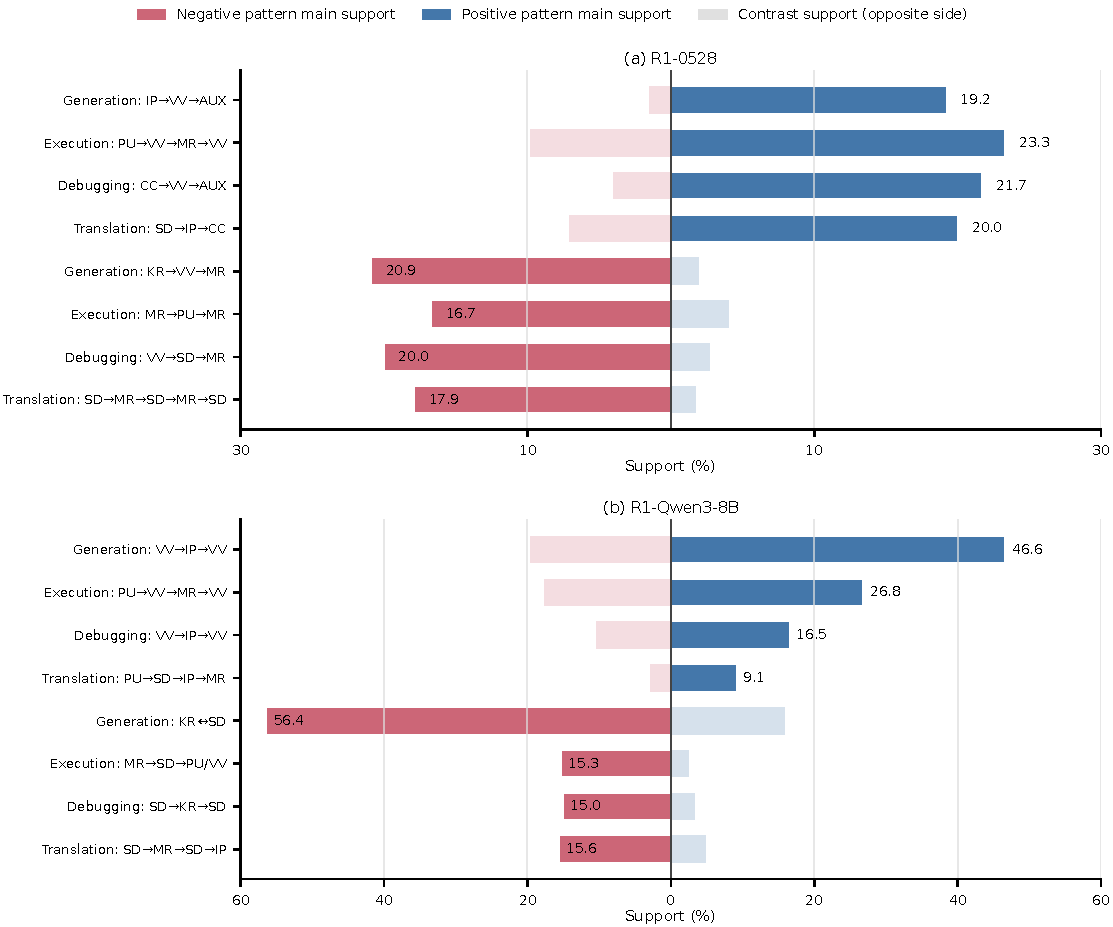
\includegraphics[width=\linewidth]{figures/rq2_valid_invalid_patterns.pdf}
\caption{Support comparison of micro reasoning patterns and anti-patterns.}
\label{fig:rq2-patterns}
\end{figure}

\subsubsection{\textbf{Micro Patterns Distinguish Productive Iteration from Reopening}}

We next examine whether these shifts are reflected in fine-grained local structures. Table~\ref{tab:rq2-pattern-catalog} summarizes the discovered micro patterns and anti-patterns, while Figure~\ref{fig:rq2-patterns} visualizes support contrasts of representative high-support patterns across task--model settings.
The results show that these differences are also manifested at the micro-pattern level. For instance, in R1-Qwen3-8B on code generation, the positive pattern \(VV \rightarrow IP \rightarrow VV\) appears in 46.6\% of valid traces but only 19.6\% of invalid traces. In contrast, the anti-pattern \(KR \leftrightarrow SD\) appears in 56.4\% of invalid traces but only 15.9\% of valid traces. Similarly, for R1-0528 on debugging, the pattern \(CC \rightarrow VV \rightarrow AUX\) is substantially more frequent in valid traces (21.7\% vs. 4.0\%), whereas \(VV \rightarrow SD \rightarrow MR\) is strongly associated with invalid traces (20.0\% vs. 2.7\%).

These patterns reveal a clear distinction in iterative behavior. Productive iteration typically follows a verify–adjust–reverify or verify–commit structure, consistent with prior findings that execution and self-verification improve reliability in code reasoning~\cite{codecot}. In contrast, invalid traces exhibit repetitive transitions centered on design revision (\(SD\)), reflection (\(MR\)), or knowledge recall (\(KR\)), without progressing toward implementation or closure.

We further check representative support contrasts using two-sided Fisher's exact tests with Benjamini--Hochberg correction, and report the complete support, count, \(p\)-value, and \(q\)-value evidence in the replication package. These results suggest that iteration per se is not predictive of correctness; rather, its target and direction determine whether it is productive or degenerative.

\subsubsection{\textbf{Cross-model Consistency with Task-dependent Strength}}
Finally, we examine the generality of the observed validity contrast across models and tasks. The closure-versus-reopening distinction is consistent across both R1-0528 and R1-Qwen3-8B, indicating that the identified reasoning patterns are not model-specific artifacts.

However, the strength of this contrast varies across settings. It is more pronounced in R1-Qwen3-8B, where invalid traces exhibit stronger cycles of design revision, reflection, and knowledge recall, suggesting that failure arises not from a lack of reasoning steps, but from persistent non-convergent exploration.

Across tasks, the effect is strongest in code generation, where invalid traces are substantially longer (17,163 vs. 7,102 tokens for R1-0528; 14,925 vs. 8,598 for R1-Qwen3-8B) and heavily concentrated in drift-oriented behaviors. Code execution and debugging tasks exhibit similar but more structured patterns, while translation shows weaker and less symmetric differences, making it a less definitive case for behavioral separation.

\begin{tcolorbox}[width=\linewidth, boxrule=0.8pt, left=2pt, right=2pt, top=2pt, bottom=2pt, colback=gray!10, colframe=black]
\textbf{Finding 2.}
Valid and invalid reasoning traces differ less in length than in their micro patterns and anti-patterns, with valid traces showing verification-driven convergence and invalid traces exhibiting anti-patterns of repeated design, reflection, and knowledge recall without closure.
\end{tcolorbox}

\section{RQ3: Applications of  Reasoning Patterns}
\label{sec:rq3}

To assess the practical utility of the discovered reasoning patterns for efficient AI coding, we conduct a set of targeted studies across code-related tasks.
\begin{itemize}
    \item \textbf{RQ3.1} \textit{Are reasoning patterns discriminative enough to distinguish different AI coding tasks? (Section \ref{sec:RQ3.1})}

    \item \textbf{RQ3.2} \textit{Can pattern-guided prompting improve task performance under comparable token budgets? (Section \ref{sec:RQ3.2})}

    \item \textbf{RQ3.3} \textit{Can pattern-aware early stopping reduce reasoning cost while preserving correctness? (Section \ref{sec:RQ3.3})}
\end{itemize}

\subsection{Task Classification from Macro-pattern Features}
\label{sec:RQ3.1}

\textbf{Setup.}
Following the task recovery probe defined in Section~\ref{sec:pattern-applications}, RQ3.1 evaluates whether task identity can be inferred from reasoning-pattern features alone. The test set consists of 3{,}376 reasoning traces generated by two models across four coding tasks. We evaluate two standard classifiers, logistic regression and random forest, using 5-fold stratified cross-validation. Performance is measured in terms of classification accuracy, reported as mean and standard deviation across folds; the random baseline is 25\% for the four-class setting.

\textbf{Results.}
Figure~\ref{fig:rq3-task-separability} reports task classification performance using only reasoning-pattern features derived from action traces. Error bars indicate cross-validation standard deviation, and the dashed line denotes the random baseline (25\%).

\begin{figure}[t]
\centering
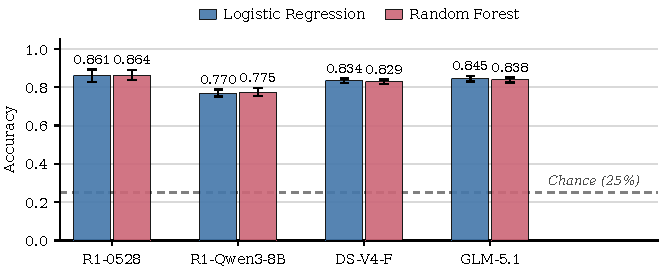
\includegraphics[width=0.8\linewidth]{figures/rq3_task_classification.pdf}
\caption{Task identification from reasoning pattern features.}
\label{fig:rq3-task-separability}
\end{figure}

Using 57 reasoning-pattern features, logistic regression achieves $0.861\pm0.032$ accuracy for R1-0528 and $0.770\pm0.019$ for R1-Qwen3-8B. Random forest yields comparable results ($0.864\pm0.027$ and $0.775\pm0.022$, respectively), indicating that task separability is robust across model families and classifiers. Since the models operate solely on reasoning-pattern features without access to task descriptions or outputs, these results demonstrate that reasoning traces preserve task identity in their structural pattern organization.

To understand which aspects of reasoning patterns drive this separability, we examine feature importance based on mutual information. For both models, the most informative features consistently relate to how reasoning effort is distributed across core actions (e.g., design ratio, and the distributions of \(PU\), \(SD\), \(IP\), and \(VV\)).
Overall, task separability is primarily driven by how reasoning traces allocate and transition reasoning effort across key functional stages rather than by trace length alone, although length provides a secondary signal.

\begin{tcolorbox}[width=\linewidth, boxrule=0.8pt, left=2pt, right=2pt, top=2pt, bottom=2pt, colback=gray!10, colframe=black]
\textbf{Finding 3.1.}
Reasoning-pattern features alone are sufficient to identify coding tasks with high accuracy, despite not using task content, answers, or metadata, suggesting that action traces inherently encode task-discriminative reasoning structures.
\end{tcolorbox}

\subsection{Micro-Pattern Guided Prompting}
\label{sec:RQ3.2}

\textbf{Setup.}
RQ3.2 explores whether micro reasoning patterns can be operationalized as inference-time guidance to improve coding performance.
We compare two prompting strategies: a \textit{default prompt}, which uses the original task instruction without additional guidance, and a \textit{pattern-guided prompt}, which augments the same instruction with task-specific guidance derived from mined micro patterns.

We apply both prompting strategies to R1-0528 and R1-Qwen3-8B across four coding tasks with objective correctness oracles. To evaluate generalizability, we further replicate the same protocol on two additional models, DeepSeek-V4-Flash (DS-V4-F)~\cite{deepseekv4} and GLM-5.1~\cite{glm51}.

Performance is measured using pass@1~\cite{codex}. To reduce variance from stochastic decoding, each setting is run three times, and we report mean pass@1 as the average across independent runs. We additionally report average per-instance token consumption (in thousands) to quantify inference cost.

\textbf{Results.}
Table~\ref{tab:rq3-prompting} summarizes the effectiveness of micro-pattern guided prompting across four AI coding tasks. We evaluate two settings: \textit{Direct}, which applies patterns mined from the same model, and \textit{Transferred}, which applies patterns mined from R1-0528 to unseen models (DS-V4-F and GLM-5.1).

\begin{table}[t!]
\centering
\caption{Pattern-Guided Prompting Results and Cross-Model Transfer. \textit{Direct} applies each model's own pattern inventory, whereas \textit{Transferred} applies pattern inventories mined from the R1 models to the previously unseen models DS-V4-F and GLM-5.1. P@1: Pass@1, measuring coding performance; Tok.: mean generated-output tokens per instance (thousands).}
\label{tab:rq3-prompting}
\papertablestyle
\setlength{\tabcolsep}{6pt}
\renewcommand{\arraystretch}{1.0}
%\resizebox{\columnwidth}{!}{%
\begin{tabular}{ll *{8}{r}}
\toprule
& & \multicolumn{4}{c}{Direct} & \multicolumn{4}{c}{Transferred} \\
\cmidrule(lr){3-6}\cmidrule(lr){7-10}
Task & Method & \multicolumn{2}{c}{R1-0528} & \multicolumn{2}{c}{R1-Qwen3-8B} & \multicolumn{2}{c}{DS-V4-F} & \multicolumn{2}{c}{GLM-5.1} \\
\cmidrule(lr){3-4}\cmidrule(lr){5-6}\cmidrule(lr){7-8}\cmidrule(lr){9-10}
 &  & P@1$\uparrow$ & Tok.$\downarrow$ & P@1$\uparrow$ & Tok.$\downarrow$ & P@1$\uparrow$ & Tok.$\downarrow$ & P@1$\uparrow$ & Tok.$\downarrow$ \\
\midrule
\multirow{4}{*}{Generation}
 & Default & 72.46 & 14.9 & 56.21 & 17.9 & 80.78 & 13.0 & 90.29 & 16.5 \\
 & {Positive-only} & {73.14} & {15.2} & {55.86} & {18.3} & {84.36} & {13.5} & {90.06} & {13.2} \\
 & {Negative-only} & {72.08} & {14.6} & {56.39} & {17.6} & {79.84} & {12.5} & {90.74} & {13.0} \\
 & PN guidance & \textbf{74.49} & 15.6 & \textbf{56.88} & 17.3 & \textbf{87.80} & 12.2 & \textbf{91.17} & 12.9 \\
\midrule
\multirow{4}{*}{\makecell{Execution\\Reasoning}}
 & Default & 55.76 & 1.7 & 44.24 & 3.4 & 56.81 & 2.1 & 59.84 & 1.6 \\
 & {Positive-only} & {57.16} & {2.4} & {48.17} & {4.4} & {58.21} & {2.6} & {60.32} & {1.6} \\
 & {Negative-only} & {56.63} & {2.1} & {46.86} & {3.9} & {57.54} & {2.3} & {60.41} & {1.5} \\
 & PN guidance & \textbf{58.37} & 2.9 & \textbf{49.74} & 4.7 & \textbf{59.27} & 2.8 & \textbf{60.73} & 1.5 \\
\midrule
\multirow{4}{*}{Debugging}
 & Default & 88.80 & 4.5 & 61.20 & 7.7 & 91.40 & 2.4 & 93.00 & 2.8 \\
 & {Positive-only} & {91.20} & {5.8} & {61.54} & {7.8} & {90.92} & {2.5} & {93.02} & {2.6} \\
 & {Negative-only} & {90.47} & {5.1} & {61.08} & {7.6} & {92.18} & {2.2} & {93.11} & {2.6} \\
 & PN guidance & \textbf{94.60} & 6.6 & \textbf{61.72} & 7.9 & \textbf{92.80} & 2.3 & \textbf{93.20} & 2.5 \\
\midrule
\multirow{4}{*}{Translation}
 & Default & 55.08 & 5.7 & 39.09 & 4.2 & 55.05 & 2.1 & 56.97 & 2.5 \\
 & {Positive-only} & {56.81} & {6.5} & {42.51} & {4.4} & {54.73} & {2.2} & {58.03} & {2.4} \\
 & {Negative-only} & {57.44} & {6.2} & {43.27} & {4.3} & {56.73} & {1.8} & {58.52} & {2.4} \\
 & PN guidance & \textbf{58.78} & 7.3 & \textbf{44.14} & 4.5 & \textbf{57.44} & 1.9 & \textbf{58.75} & 2.3 \\
\bottomrule
\end{tabular}
%}
\end{table}

\FloatBarrier

\textit{1) Direct Results.}
Pattern-guided prompting improves mean pass@1 on all four tasks for both R1-0528 and R1-Qwen3-8B, with the largest gains on debugging for R1-0528 and on execution reasoning and translation for R1-Qwen3-8B\textcolor{blue}{ (+5.80, +5.50, and +5.05 points, respectively)}.

Improvement is task-dependent, \textcolor{blue}{tending to be larger on tasks with clearer separation between the positive patterns and anti-patterns identified in RQ2}. Token consumption remains comparable to the default \textcolor{blue}{prompt, suggesting that the gains do not merely stem} from longer reasoning. These results \textcolor{blue}{indicate} that structured positive and negative cues improve correctness without revealing task-specific solutions.

\textcolor{blue}{\textit{2) Ablation: Positive Patterns vs.\ Anti-pattern Constraints.}
To isolate the contribution of each guidance component, we further evaluate two ablated variants: \textit{Pattern-only}, which retains only the positive patterns mined from valid traces, and \textit{Anti-pattern-only}, which retains only the negative constraints derived from anti-patterns.
Across the twelve task--model settings where ablations are available, each component alone yields inconsistent gains and can even underperform the default prompt: Pattern-only degrades R1-Qwen3-8B generation (55.86 vs.\ 56.21) and DS-V4-F translation (54.73 vs.\ 55.05), while Anti-pattern-only degrades DS-V4-F generation (79.84 vs.\ 80.78) and R1-Qwen3-8B debugging (61.08 vs.\ 61.20). In contrast, their combination achieves the highest pass@1 among all guided variants in every task--model setting and surpasses the default prompt in all settings except GLM-5.1 generation.
This complementarity is consistent with the RQ2 findings: positive patterns steer reasoning toward verification-driven closure (e.g., \(VV\rightarrow IP\rightarrow VV\)), whereas anti-pattern constraints suppress drift-oriented reopening loops (e.g., \(SD\rightarrow KR\rightarrow SD\)). Each ablated variant covers only one side of this contrast: Pattern-only steers reasoning toward closure but leaves the reopening loops unguarded, so reasoning can still drift into the failure modes that RQ2 associates with invalid traces. Conversely, Anti-pattern-only suppresses these loops but offers no constructive direction, so avoiding known failure loops does not by itself ensure productive closure. Combining the two addresses both sides and yields stable improvements.}

\textit{3) Transferred Results.}
Pattern-guided prompting further generalizes to unseen models. On DS-V4-F, improvements are observed \textcolor{blue}{on all four tasks, with the largest gain on code generation (+7.02 points)}, with token usage remaining stable relative to the default prompt. On GLM-5.1, performance improves on execution reasoning, debugging, and translation, with only a minor decrease on code generation\textcolor{blue}{ (--1.13 points), which we attribute to its near-saturated default accuracy (90.29\%) that leaves limited headroom for external guidance; nonetheless, token consumption drops substantially (16.5K$\rightarrow$12.9K), suggesting that the guidance accelerates convergence even when correctness is saturated}. The transferred gains suggest that the mined micro patterns are model-agnostic rather than specific to the R1 family.

\begin{tcolorbox}[width=\linewidth, boxrule=0.8pt, left=2pt, right=2pt, top=2pt, bottom=2pt, colback=gray!10, colframe=black]
\textbf{Finding 3.2.}
Micro-pattern-guided prompts that integrate positive patterns and anti-patterns consistently improve mean pass@1 across tasks under comparable token cost and generalize to held-out models\textcolor{blue}{, with the two guidance components being individually unstable but jointly complementary}, suggesting that reasoning patterns provide transferable, solution-agnostic guidance for improving coding performance.
\end{tcolorbox}

\subsection{Pattern-aware Early Stopping}
\label{sec:RQ3.3}

\textbf{Setup.} 
RQ3.3 examines whether anti-pattern signals can be leveraged for online early stopping to reduce inference cost while preserving correctness.
We compare two settings: \emph{Full Reasoning}, which allows the model to complete its full reasoning process before producing an answer, and \emph{Pattern-aware Stop}, an online stopping policy defined in Section~\ref{sec:pattern-applications} that monitors the streaming reasoning trace and triggers early termination once sufficient drift signals are detected.
Since Pattern-aware Stop requires access to streaming reasoning outputs, we apply it to R1-Qwen3-8B and the two held-out generalization models, while R1-0528 is excluded due to the lack of a streaming-capable interface during evaluation.
Following RQ3.2, each setting is executed three times, and we report mean pass@1 together with the average token consumption per instance as a measure of inference cost.

\begin{table}[t]
\centering
\caption{Pattern-aware Early Stopping Performance across Models}
\label{tab:rq3-early-stopping}
\scriptsize
\setlength{\tabcolsep}{2.5pt}
\renewcommand{\arraystretch}{1.08}
\resizebox{\columnwidth}{!}{%
\begin{tabular}{@{}llcccc@{}}
\toprule
\multirow{2}{*}{Task} & \multirow{2}{*}{Model} & \multicolumn{2}{c}{Full Reasoning} & \multicolumn{2}{c}{Pattern-aware Stop} \\
\cmidrule(lr){3-4}\cmidrule(lr){5-6}
 & & P@1 & Tok. & P@1 & Tok. \\
\midrule
\multirow{3}{*}{Generation}
 & R1-Qwen3-8B & 56.21 & 17.89K & 52.14 \textcolor{red!70!black}{\scriptsize(--4.07)} & 10.64K \textcolor{green!50!black}{\scriptsize(--40.56\%)} \\
 & DS-V4-F & 80.78 & 13.00K & 73.36 \textcolor{red!70!black}{\scriptsize(--7.42)} & 8.43K \textcolor{green!50!black}{\scriptsize(--35.13\%)} \\
 & GLM-5.1 & 90.29 & 16.54K & 88.06 \textcolor{red!70!black}{\scriptsize(--2.23)} & 7.85K \textcolor{green!50!black}{\scriptsize(--52.52\%)} \\
\midrule
\multirow{3}{*}{\makecell{Execution\\Reasoning}}
 & R1-Qwen3-8B & 44.24 & 3.43K & 40.58 \textcolor{red!70!black}{\scriptsize(--3.66)} & 2.10K \textcolor{green!50!black}{\scriptsize(--38.75\%)} \\
 & DS-V4-F & 56.81 & 2.13K & 51.57 \textcolor{red!70!black}{\scriptsize(--5.24)} & 0.85K \textcolor{green!50!black}{\scriptsize(--59.78\%)} \\
 & GLM-5.1 & 59.84 & 1.64K & 58.63 \textcolor{red!70!black}{\scriptsize(--1.21)} & 0.52K \textcolor{green!50!black}{\scriptsize(--68.53\%)} \\
\midrule
\multirow{3}{*}{Debugging}
 & R1-Qwen3-8B & 61.20 & 7.65K & 54.40 \textcolor{red!70!black}{\scriptsize(--6.80)} & 4.18K \textcolor{green!50!black}{\scriptsize(--45.32\%)} \\
 & DS-V4-F & 91.40 & 2.42K & 86.60 \textcolor{red!70!black}{\scriptsize(--4.80)} & 1.69K \textcolor{green!50!black}{\scriptsize(--30.16\%)} \\
 & GLM-5.1 & 93.00 & 2.77K & 91.20 \textcolor{red!70!black}{\scriptsize(--1.80)} & 1.74K \textcolor{green!50!black}{\scriptsize(--37.16\%)} \\
\midrule
\multirow{3}{*}{Translation}
 & R1-Qwen3-8B & 39.09 & 4.18K & 37.64 \textcolor{red!70!black}{\scriptsize(--1.45)} & 2.33K \textcolor{green!50!black}{\scriptsize(--44.22\%)} \\
 & DS-V4-F & 55.05 & 2.14K & 50.79 \textcolor{red!70!black}{\scriptsize(--4.26)} & 1.23K \textcolor{green!50!black}{\scriptsize(--42.65\%)} \\
 & GLM-5.1 & 56.97 & 2.53K & 55.48 \textcolor{red!70!black}{\scriptsize(--1.49)} & 1.51K \textcolor{green!50!black}{\scriptsize(--40.56\%)} \\
\bottomrule
\end{tabular}
}
\end{table}

\FloatBarrier

\textbf{Results.} 
Table~\ref{tab:rq3-early-stopping} summarizes the effectiveness of pattern-aware early stopping across four AI coding tasks. On R1-Qwen3-8B, the stopping policy consistently reduces token consumption by 38.75\%--45.32\%, with pass@1 reductions of 1.45 to 6.80 points. The cost--accuracy trade-off is task-dependent: translation exhibits the most favorable balance (44.22\% token reduction with only a 1.45-point drop), whereas generation and debugging incur larger accuracy degradation at comparable savings, suggesting these tasks more often require extended reasoning before convergence.

We observe a similar trend on held-out models DS-V4-F and GLM-5.1, which were not involved in pattern mining. On DS-V4-F, the policy reduces token cost by 30.16\%--59.78\%, with the largest accuracy loss on generation (--7.42 points) but a more balanced trade-off on debugging. On GLM-5.1, token savings reach 37.16\%--68.53\% with small accuracy drops (1.21--2.23 points). These results demonstrate that pattern-aware early stopping generalizes beyond the models used for pattern discovery, while consistently exposing a controllable cost--correctness trade-off.

\begin{tcolorbox}[width=\linewidth, boxrule=0.8pt, left=2pt, right=2pt, top=2pt, bottom=2pt, colback=gray!10, colframe=black]
\textbf{Finding 3.3.}
Pattern-aware early stopping achieves substantial token cost reduction (30--69\%) with limited accuracy degradation (1.21--7.42 percentage-point pass@1 drop) across task--model settings, and generalizes across models.
%The stopping policy, derived from RQ2 anti-patterns, transfers to DS-V4-F without modification, indicating cross-model generalizability of failure-associated drift characteristics.
\end{tcolorbox}

\section{Discussion}
\subsection{Understanding Reasoning Structures}

Our results suggest that reasoning in AI coding is organized around recurrent action-level structures rather than isolated step sequences or linear chains of thought. Across tasks, we observe stable macro-level behavioral regularities, indicating that reasoning traces exhibit compositional structure that is consistent within tasks but distinct across them.

At a finer granularity, the contrast between valid and invalid traces suggests that reasoning quality is closely related to how actions evolve toward convergence. This is reflected in the identified micro-level patterns and anti-patterns, which capture differences in action-level progression between successful and unsuccessful trajectories.

\subsection{Future Research Directions}

Our findings suggest several promising directions for future research on reasoning in AI coding.

\subsubsection{Evaluation of Reasoning Models}
Reasoning traces provide structured behavioral signals that are not captured by outcome-based metrics such as pass@1 or trace length. This motivates future work on evaluation frameworks grounded in action-level reasoning structure, enabling finer-grained assessment of model reasoning behavior.

\subsubsection{Structure-Aware Inference Control}
The discovered reasoning patterns suggest the potential for controlling inference through structural signals, enabling fine-grained monitoring and intervention during reasoning, including but not limited to early stopping.

\subsubsection{Learning with Reasoning Structure}
Beyond pattern-guided prompting, pattern-augmented reasoning traces expose intermediate structures that may serve as supervision signals for training models that explicitly optimize reasoning processes.

\section{Threats to Validity}

\textbf{Construct Validity.}
Our analysis abstracts free-form reasoning traces into discrete reasoning actions, enabling systematic comparison but potentially losing fine-grained semantic distinctions and internal reasoning nuances. We mitigate this limitation by grounding the taxonomy in prior work, refining it via expert inspection, and validating automatic annotations against human re-labeling (Cohen’s $\kappa=0.816$). However, alternative taxonomies, segmentation granularities, or collapsing rules may lead to different  patterns, suggesting the need for sensitivity analysis in future work.

\textbf{Internal Validity.}
Validity labels are derived from an LLM-based judge ensemble and task-level pass@1, which may still miss subtle reasoning errors or overestimate correctness. We reduce this risk using confidence-weighted voting, human adjudication of low-confidence cases, and objective correctness oracles. Nonetheless, prompting and early-stopping results should be interpreted as intervention evidence rather than causal attribution to specific mined patterns, motivating future controlled interventions for causal validation.

\textbf{External Validity.}
Our study spans four coding tasks and four LRMs, which may not fully represent the diversity of software engineering scenarios or model architectures. While we evaluate both in-distribution and held-out models, further validation across tasks, languages, and model families is required to assess generality.

\section{Related Work}

Recent LRMs incorporate extended reasoning traces as a core component of inference~\cite{deepseekr1}. In code-related settings, prior work shows that reasoning-before-coding is not uniformly beneficial and depends on how reasoning is structured relative to code generation~\cite{revisitcotcodegen}. Other studies explore leveraging external or structured signals to improve reasoning, such as mining discussion data into training chains~\cite{svrc2026} or validating intermediate steps via search-based refinement~\cite{mctsrefine2025}. These efforts demonstrate the utility of explicit reasoning for code generation, but primarily focus on improving outputs or training signals rather than characterizing recurring reasoning structures across tasks.

Prior work also examines reasoning quality and failure modes. Studies show that reasoning quality is not reliably aligned with final correctness, as flawed reasoning may still produce correct outputs and vice versa~\cite{cotcodequality}, and that superficial signals such as step count or verbosity are weak indicators of correctness~\cite{reasoningsteps2026}. Recent work further categorizes reasoning behaviors and failure patterns such as hallucination, overthinking, and erroneous backtracking~\cite{thinkingpatterns,reasoninghallucination2025,demystifyingerrors2025}. While these studies move beyond outcome-only evaluation, they are often limited to single tasks or rely on coarse-grained or manual annotations, leaving open how reasoning structures vary across tasks and how they differ between valid and invalid traces.

Reasoning traces have also been studied for inference-time control. Methods such as SEER adapt reasoning strategies during generation~\cite{seer2025}, while work on overthinking motivates compressing redundant reasoning steps~\cite{overthinking2025,asap2025,adaptivecot2025}. Early-stopping approaches exploit intermediate signals to terminate generation based on convergence or confidence criteria~\cite{answerconvergence2025,deer2026}. These methods primarily optimize efficiency or decoding behavior, but do not explicitly derive reasoning patterns from empirical trace analysis.

In contrast, we treat reasoning traces as empirical behavioral artifacts, abstracting them into reasoning action traces and analyzing recurring structures across code generation, code execution reasoning, program debugging, and code translation. This enables a unified characterization of task-level patterns and action-level (anti-)patterns, and further connects these structures to downstream applications in task identification, pattern-guided prompting, and pattern-aware early stopping.

\section{Conclusion}
In this paper, we present an empirical study of reasoning patterns in AI coding. By abstracting reasoning traces into action sequences, we identify macro-level patterns that characterize task-specific reasoning strategies and micro-level patterns that distinguish effective from ineffective reasoning across four coding tasks. We further show that these patterns are actionable, enabling task identification, improved prompting, and token-efficient inference via early stopping, positioning reasoning patterns as a practical abstraction for understanding and improving the efficiency of LRMs in AI coding.

\section*{Data Availability}

All code and data used in this study are publicly available at: \url{https://anonymous.4open.science/r/ICSE_2027-2554}. %The repository includes: (i) the collected reasoning traces and annotated datasets across the four tasks (code generation, code execution reasoning, debugging, and translation); (ii) the code for  pattern discovery, pattern-guided prompting and pattern-aware early stopping (RQ1--RQ3); and (iii) all experimental results and evaluation scripts.

\bibliographystyle{ACM-Reference-Format}
\bibliography{ref}

\end{document}
